\documentclass{beamer}
\mode<presentation>
%% \mode<handout>{\setbeamercolor{background canvas}{bg=black!5}}
\usetheme{CambridgeUS}
\usecolortheme{dolphin}

\usepackage{bstyle}

\title{Statistics for a Computational Topologist}
\subtitle{Part I}
\author[B.\ Fasy]{Brittany Terese Fasy\\ TA: Samuel A.\ Micka}
\institute[MSU]{School of Computing and Dept.\ of Mathematical Sciences\\ Montana State University}
\date{\today}

\begin{document}

\begin{frame}
\titlepage
\end{frame}

\frame{
\frametitle{Why Topological Data Analysis?}
\framesubtitle{``Data has shape and the shape matters.'' - Gunnar Carlsson}
\begin{block}{}
 Today, Data is high-dimensional, \onslide<2->{HUGE,}
 \onslide<3->{present everywhere}
 \vspace{.2in}
 \begin{columns}
  \column{.32\textwidth}
 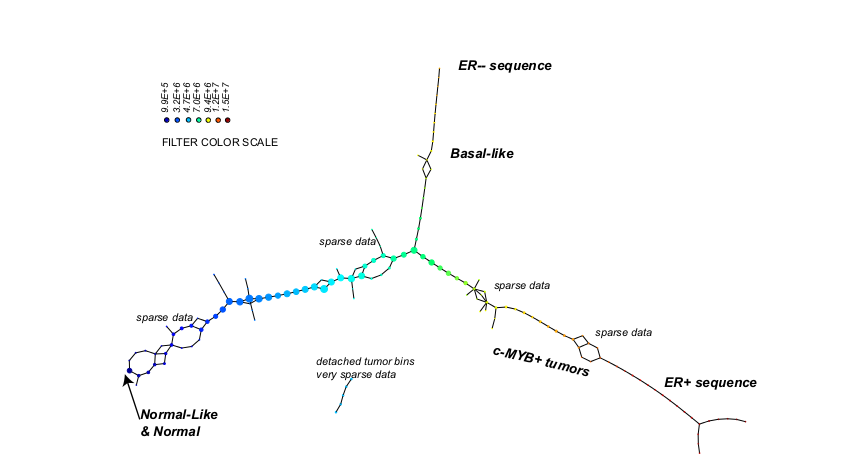
\includegraphics[width=\textwidth,height=1.25in]{examples/stanford-reeb}%
   \\
   ---------------------\\
   \scriptsize{Nicolaua, Levine, and Carlsson, PNAS 2011}
   \column{.32\textwidth}
   \onslide<2->{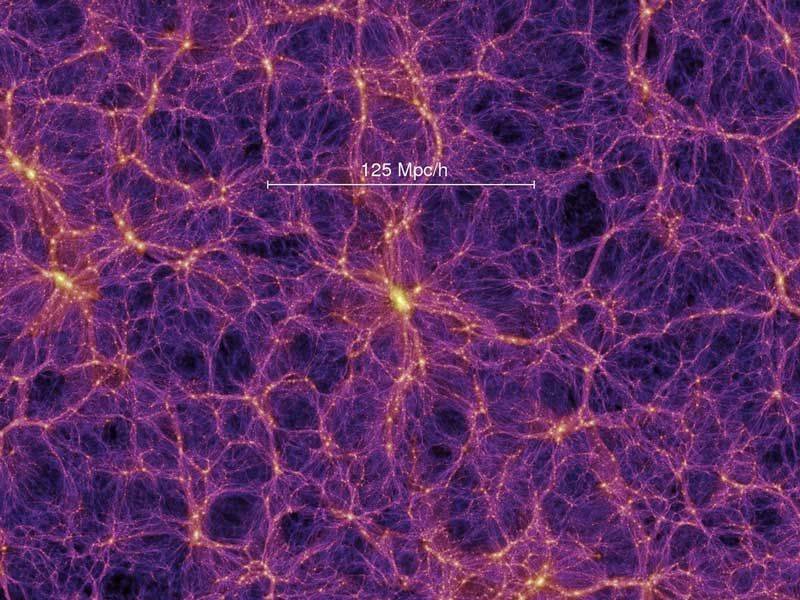
\includegraphics[width=\textwidth]{examples/cosmic-web}
   \\
   ---------------------\\
   \scriptsize{http://astrobites.com/}
   }%
   \column{.32\textwidth}
   \onslide<3->{
   \vspace{.2in} \\
   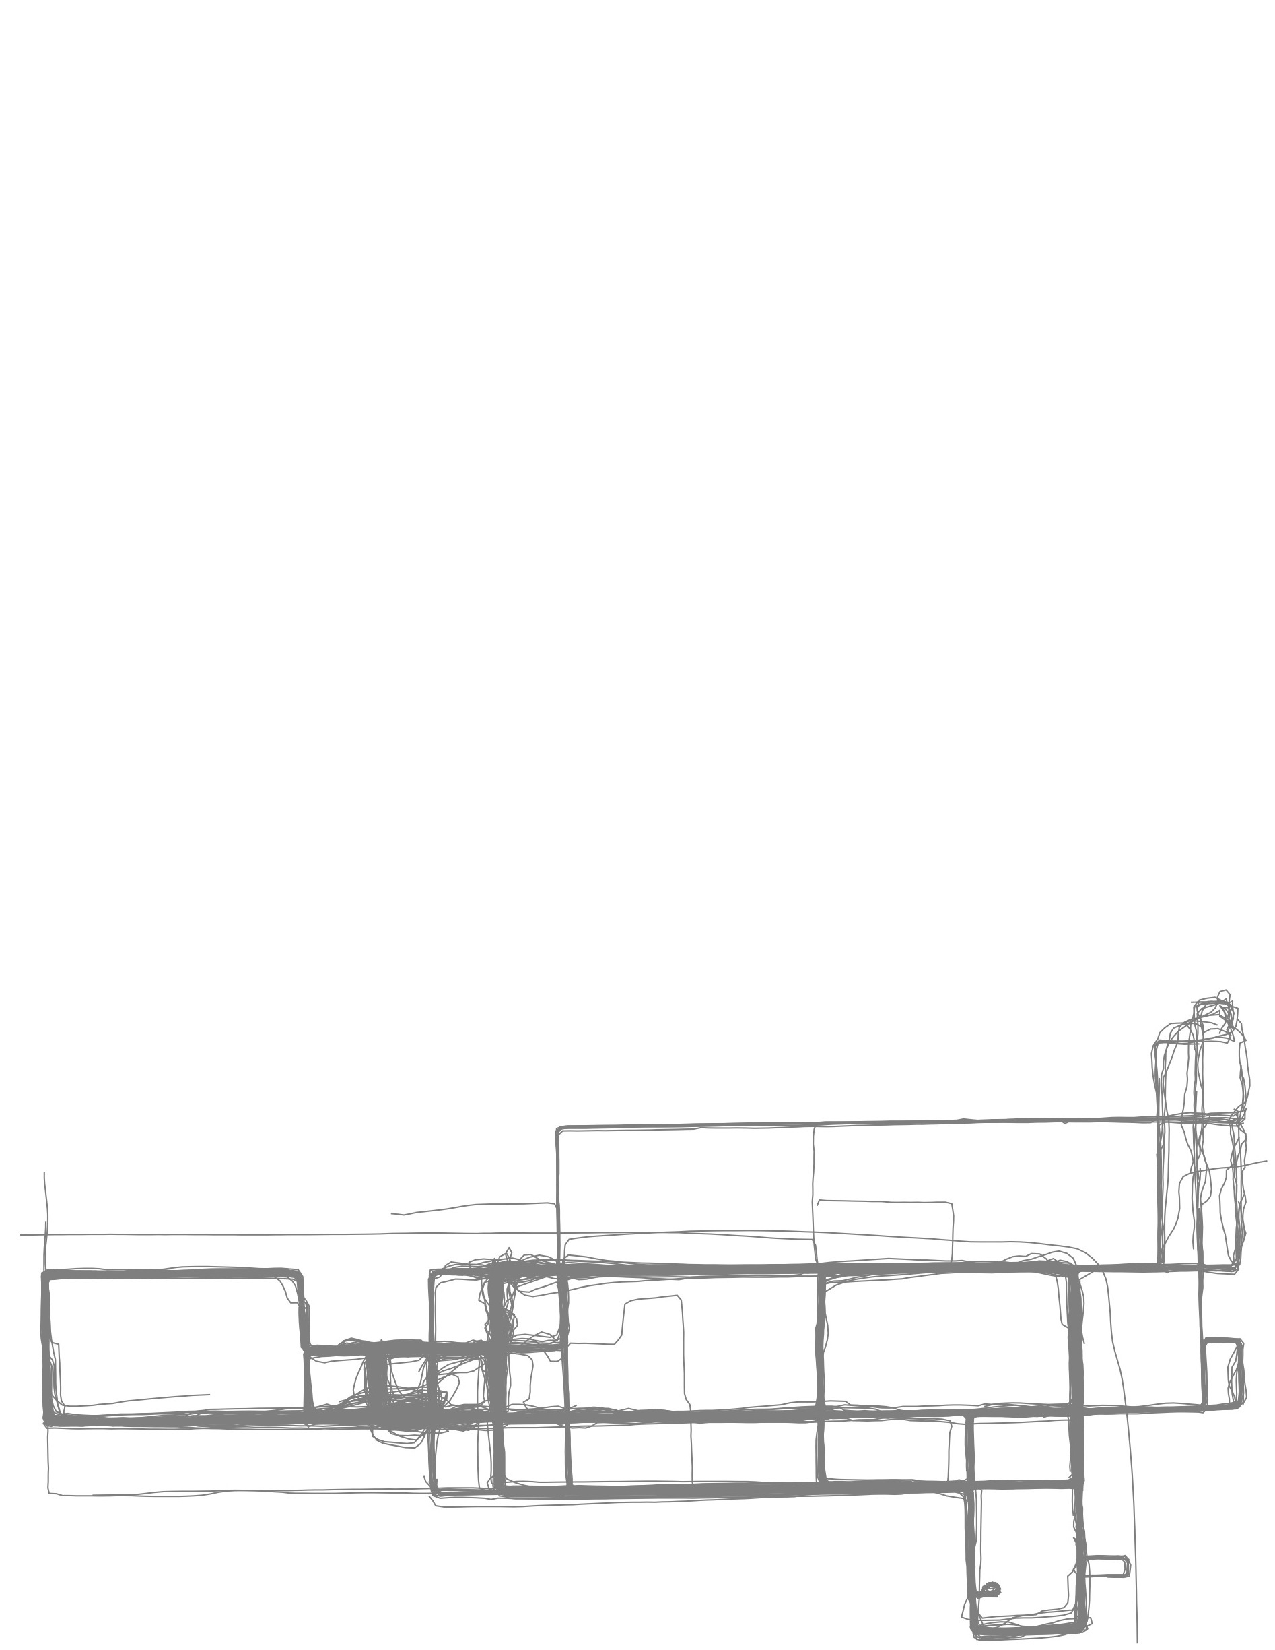
\includegraphics[width=\textwidth]{examples/chicago-tracks}
   \vspace{.2in} \\
   ---------------------\\
   \scriptsize{\url{www.mapconstruction.org}}
   }
 \end{columns}
 \vspace{.2in}
 ... and needs to be summarized, analyzed, and compared!

\end{block}
}

\frame{
    \begin{block}{\center{What questions do we ask in data anaylsis?}}
        \pause
    \begin{itemize}
        \item Think! Write down one question (2 min) \pause
        \item Pair! Share with partner, and add more questions to your list (5
            min) \pause
        \item Share! Raise hands please! (5 min) \pause
        \item More ideas? \url{mickas37@gmail.com}
    \end{itemize}
    \end{block}
}

\frame{
    \frametitle{Data Analysis Questions}
        \begin{block}{Summarize and Analyze}
            \begin{itemize}
                \item What is this shape? \pause How many components / populations?
                    \pause
                \item Can we categorize? (Classification) \pause
                \item What are the parameters? (Inference: Point Estimation)
                    \pause
                \item How far do parameters likely lie from estimates?
                    (Confidence Sets) \pause
            \end{itemize}
        \end{block}
        \begin{block}{Compare}
            \begin{itemize}
                \item Are these the same? \pause  In distribution? \pause
                \item Has something changed? \pause If so, what has changed? \pause
                \item Which is bigger? \pause
                \item Can we retain the null hypothesis? (Inference: Hypothesis
                    Testing) \pause
                \item What is the relationship between $X$ and $Y$? (Regression)
            \end{itemize}
        \end{block}
}

\frame{
    \frametitle{Most Important Questions}

    \pause
    \begin{block}{}
        1. Which descriptor best captures our data? \pause
        \begin{itemize}
            \item Descriptors
            \item Confidence Sets
        \end{itemize}
    \end{block}

    \pause
    \begin{block}{}
        2. How do we measure distance between descriptors? \pause
        \begin{itemize}
            \item Distances
            \item Clustering
        \end{itemize}
    \end{block}
}

\section{Descriptors}
\frame{
    \begin{block}{}
        \centering
        Topological Descriptors
    \end{block}
}

\frame{
    \frametitle{Stat Slide: The Basics}

    \begin{block}{}
        \begin{itemize}
            \onslide<1->{\item Let $F$ be a probability distribution with
                density $f$.}%
            \onslide<2->{\item $X \sim F$ reads ``$X$ has distribution $F$".}%
            \onslide<2->{\item $X$ is a \emph{random variable}.}
            \onslide<3->{\item Expectation: $\mathbb{E}(X) = \int x \,dF(x)$.}
            \onslide<4->{\item Quantile Function $\textsc{CDF}^{-1}(q)$.}
        \end{itemize}

            \centering
            \only<1-3>{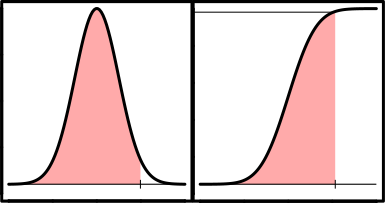
\includegraphics[width=3in]{figs/stat/pdfcdf}}%
            \only<4>{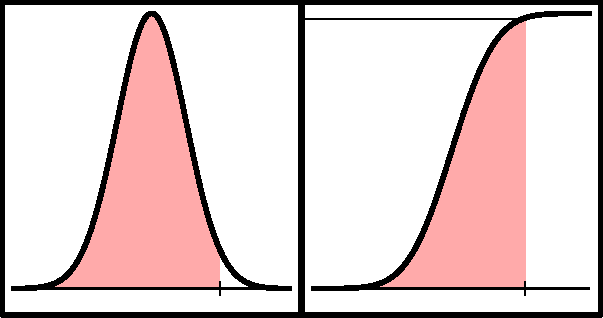
\includegraphics[width=3in]{figs/stat/pdfcdf-quantile}}%
    \end{block}
}

\frame{
    \frametitle{Prob/Stat Slide: Descriptors and Limit Theory}

    \begin{block}{}
        \begin{itemize}
            \item Let $F$ be some distribution.
            \item Let $X_1, X_2, \ldots, X_n \sim F$. (The data). \pause
            \item A \emph{statistic} or \emph{descriptor} is a function of the data:\\
                $T(X_1, X_2, \ldots, X_n)$ or $T(X^n)$. \pause
            \item Sample average: $\bar{X}^n = \frac{1}{n}\sum{X_i}$.
        \end{itemize}
    \end{block}

    \pause
    \begin{block}{Law of Large Numbers}
        $\bar{X^n}$ converges to $\mathbb{E}(X_i)$ in probability: \pause
        $$\forall \varepsilon >0, \lim_{n \to \infty} (
                |\mathbb{P}(\bar{X}^n - \mathbb{E}(X_i)| > \varepsilon) \to 0.$$
    \end{block}

    \pause
    \begin{block}{Central Limit Theorem}
        $\sqrt{n}(\bar{X}^n-\mathbb{E}(X_i))$ converges in distribution to a
        Normal distribution, \pause i.e., sample average is approximately Normal
        for large enough samples.
    \end{block}
}

\frame{
\begin{block}{}
    \frametitle{Data as Point Clouds}
\centering
 \only<1>{\includegraphics[width=\textwidth]{topology/pers-maps-circle-points}}%
 \only<2->{\includegraphics[width=\textwidth]{topology/pers-maps-circle}}%
\end{block}
}


\frame{
\begin{block}{}
\frametitle{Data as Persistence Diagrams}
\centering
 \only<1->{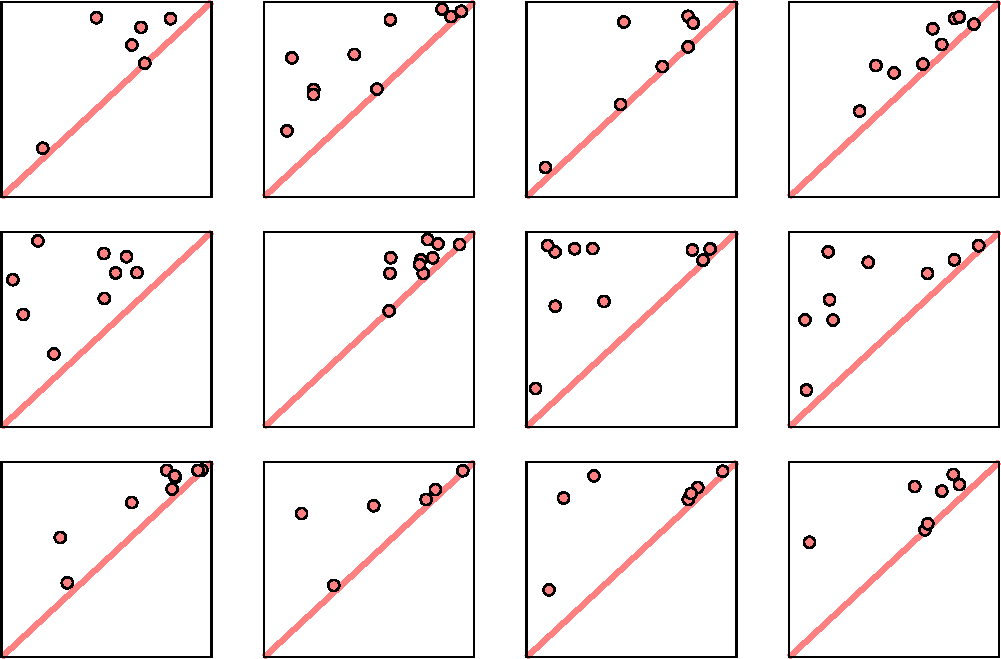
\includegraphics[width=.9\textwidth]{stat/sampling-dgms}}%
\end{block}
}


\section{Confidence Sets}
\frame{
\frametitle{}
\begin{block}{}
\centering
Confidence Sets for Persistence Diagrams:\\
Analyzing Descriptors
\end{block}
}

\frame{
\frametitle{Objective}
\framesubtitle{~}

\begin{block}{To Find a Threshold}
 Given $\alpha \in (0,1)$, we will find $q^{\alpha}$ such that
  $$\mathbb{P}(
  W_{\infty}(D,\widehat{D}_n) \leq q^{\alpha}
) \geq 1-\alpha.$$
\end{block}
\pause
\begin{block}{References}
    \begin{itemize}
        \item BTF, Lecci, Rinaldo, Wasserman, Balakrishnan, and Singh.
            Confidence sets for persistence diagrams. Annals of Stat., 2014.
        \item Chazal, BTF, Lecci, Rinaldo, Singh, and Wasserman.
            On the Bootstrap for Persistence
            Diagrams and Landscapes.
            Modeling and Analysis of Information Systems, 2013.
        \item Chazal, BTF, Lecci, Michel, Rinaldo, and Wasserman.
            Robust Topological Inference: Distance To a Measure and Kernel
            Distance, JMLR 18(159):1--40, 2018.
    \end{itemize}
\end{block}
}

\frame{
    \frametitle{Stat Slide: Bootstrapping}
    \begin{block}{}
        \begin{itemize}
            \item Old idiom: ``pull yourself up by your bootstraps" \pause
            \item Want: a parameter of an unknown distribution $F$. \pause
            \item Try: estimate using empirical distribution $\hat{F}$. \pause
            \item Nonparametric technique!
        \end{itemize}
    \end{block}
}

\begin{frame}
    \frametitle{Bottleneck Bootstrap}

    \begin{columns}
        \column{.45\textwidth}

        \begin{block}{}
            We have a point cloud sample: $\mathcal{S}_n = \{ X_1, \ldots, X_n\}$; $X_i \sim P$.
        \end{block}

        \pause

        \begin{block}{}
            Subsample (with replacement), obtaining:
            $X = \{ X_1^*, \ldots, X_b^*\}$
        \end{block}

        \pause

        \begin{block}{}
            Compute
            $\hat{\Theta}_b^*(X^*) =
            W_{\infty}(X^*,\mathcal{S}_n)$ using KDE or DTM.
        \end{block}

        \column{.45\textwidth}
        \centering
        \only<4-5>{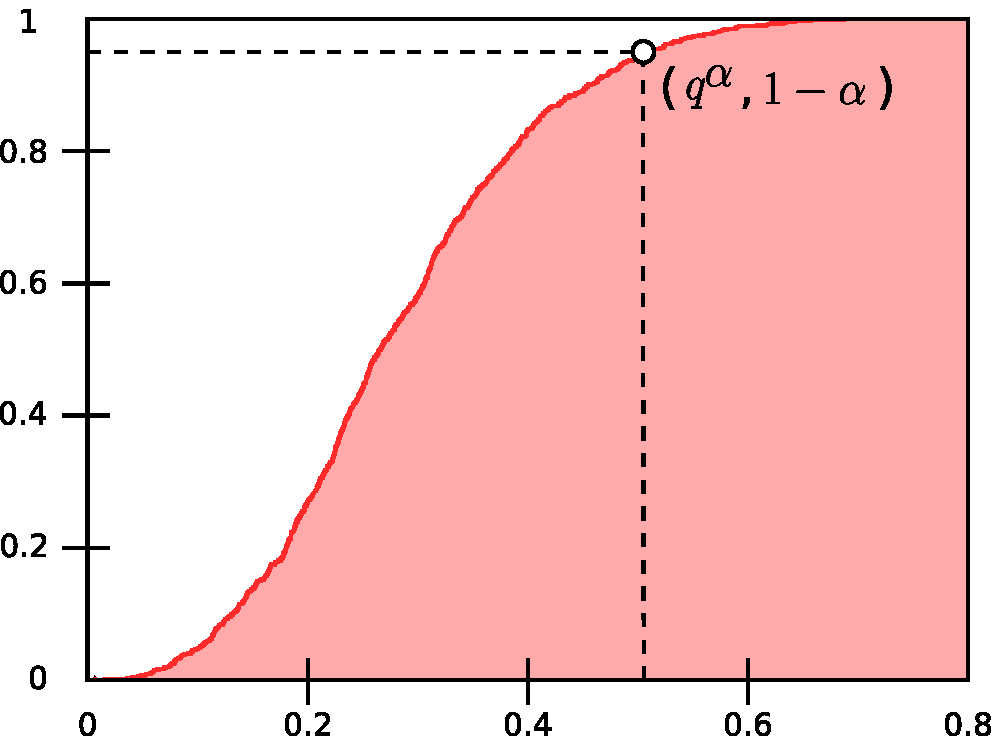
\includegraphics[height=1.6in]{stat/cdf-full}}
        \only<6->{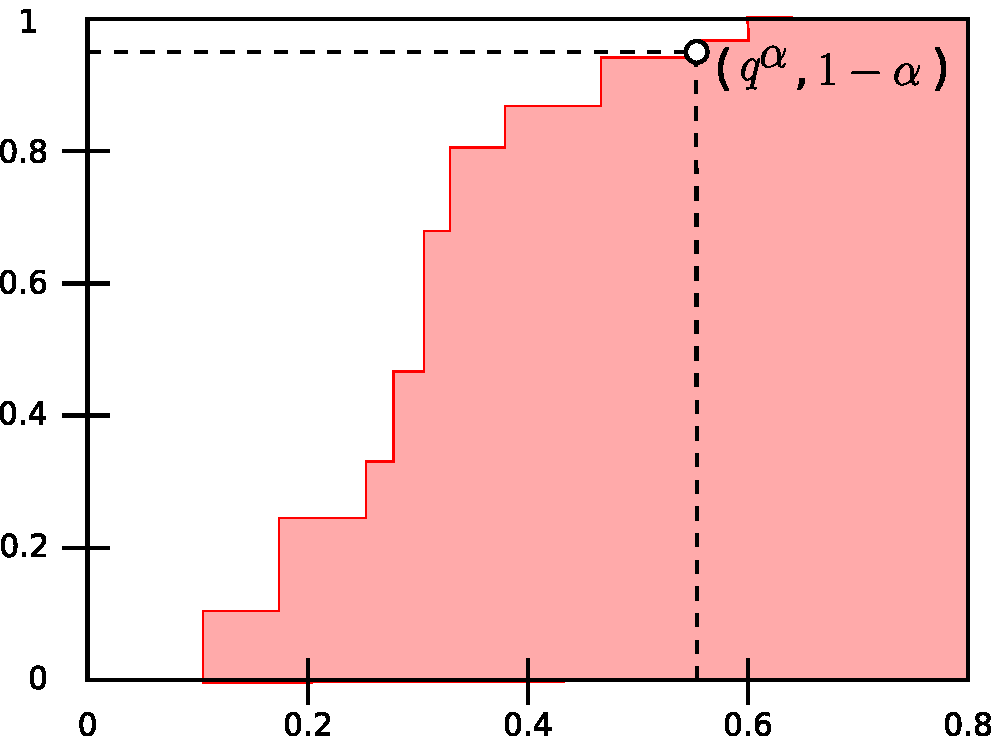
\includegraphics[height=1.6in]{stat/cdf-estimate}}

    \end{columns}

    \pause
    \begin{columns}
        \column{.45\textwidth}
        \begin{block}{}
            Consider all possible outcomes:
            $$ \{ \hat{\Theta}_{b}^*(X^*) \}_{X^* \subset \mathcal{S}_n}$$
        \end{block}

        \column{.45\textwidth}
        \pause
        \begin{block}{}
            Mimics:
            $$ \{ {\Theta}(X) = W_{\infty}(\mathcal{S}_n,\mathbb{M}) \}_{\mathcal{S}_n
            \subset \mathbb{M}}$$
        \end{block}
    \end{columns}
\end{frame}



\begin{frame}
 \frametitle{Confidence Sets for Persistent Diagrams}
 \framesubtitle{~}
 % side by side figures
 \begin{block}{}
  $$C_{\alpha}
  = \{ D \in \mathcal{D}_T ~:~ W_{\infty}(D,\widehat{D}_n) \leq q^{\alpha} \}$$
 \end{block}

 \begin{columns}
  \column{.45\textwidth}
     \begin{figure}
     \centering

 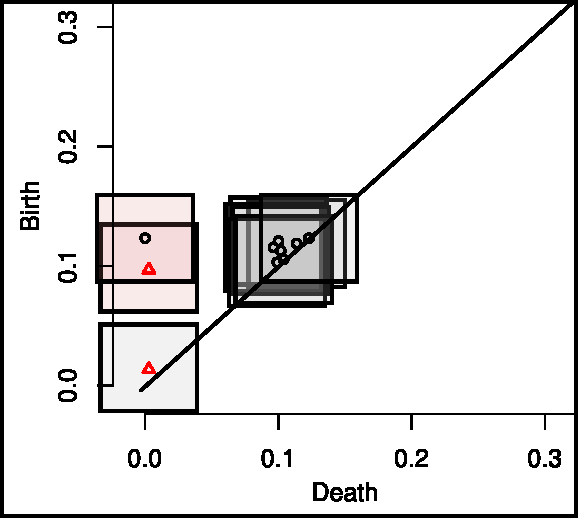
\includegraphics[height=1.6in]{stat/eyeglasses-density-pers-Point-ci.pdf}
     \end{figure}
  \column{.45\textwidth} \pause
     \begin{figure}
     \centering

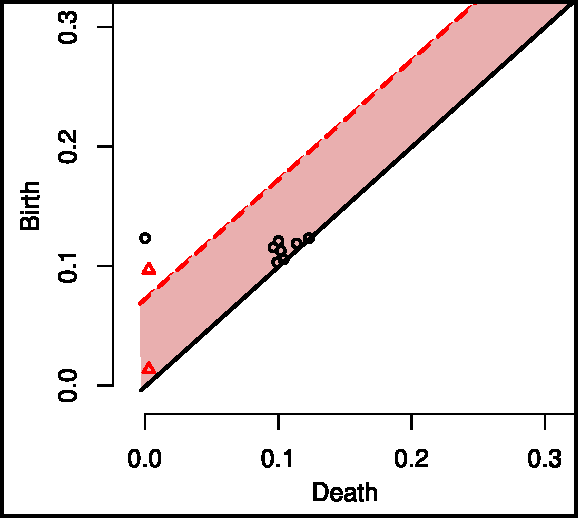
\includegraphics[height=1.6in]{stat/eyeglasses-density-pers-CI.pdf}
     \end{figure}
\end{columns}
\end{frame}

\frame{
    \frametitle{Example}

    \begin{block}{}
        \centering
        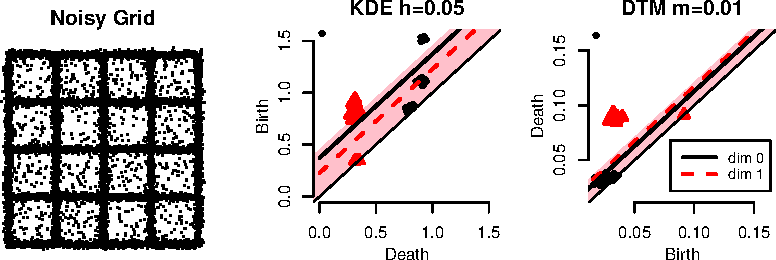
\includegraphics[width=\textwidth]{stat/noisy-grid2}
    \end{block}
}


\frame{
    \frametitle{Challenges}

    \pause
    \begin{columns}
        \column{.45\textwidth}
        \begin{block}{Techniques}
            \begin{itemize}
                \item Prove convergence rates. \pause
                \item Determine suitable assumptions on input. \pause
                \item Use the geometry of input (e.g., properties of an
                    underlying smooth manifold). \pause
            \end{itemize}
        \end{block}

        \column{.45\textwidth}
        \begin{block}{Questions}
            \begin{itemize}
               \item These results are \emph{in the limit}. When is $n$ big
                    enough? \pause
                \item What confidence sets can we construct in the multi-d
                    setting? \pause
                \item What is the optimal threshold for particular
                    filtrations? \pause
                \item Power analysis: are the rejected points topologically
                    insignificant? (Type II errors) \pause
            \end{itemize}

        \end{block}
    \end{columns}
}

\section{Distances}
\frame{
    \frametitle{}

\begin{block}{}
    \centering
    Distance Measures:\\
    Comparing Descriptors
\end{block}
}

\frame{
\frametitle{}

\begin{block}{}
\centering
 \only<1>{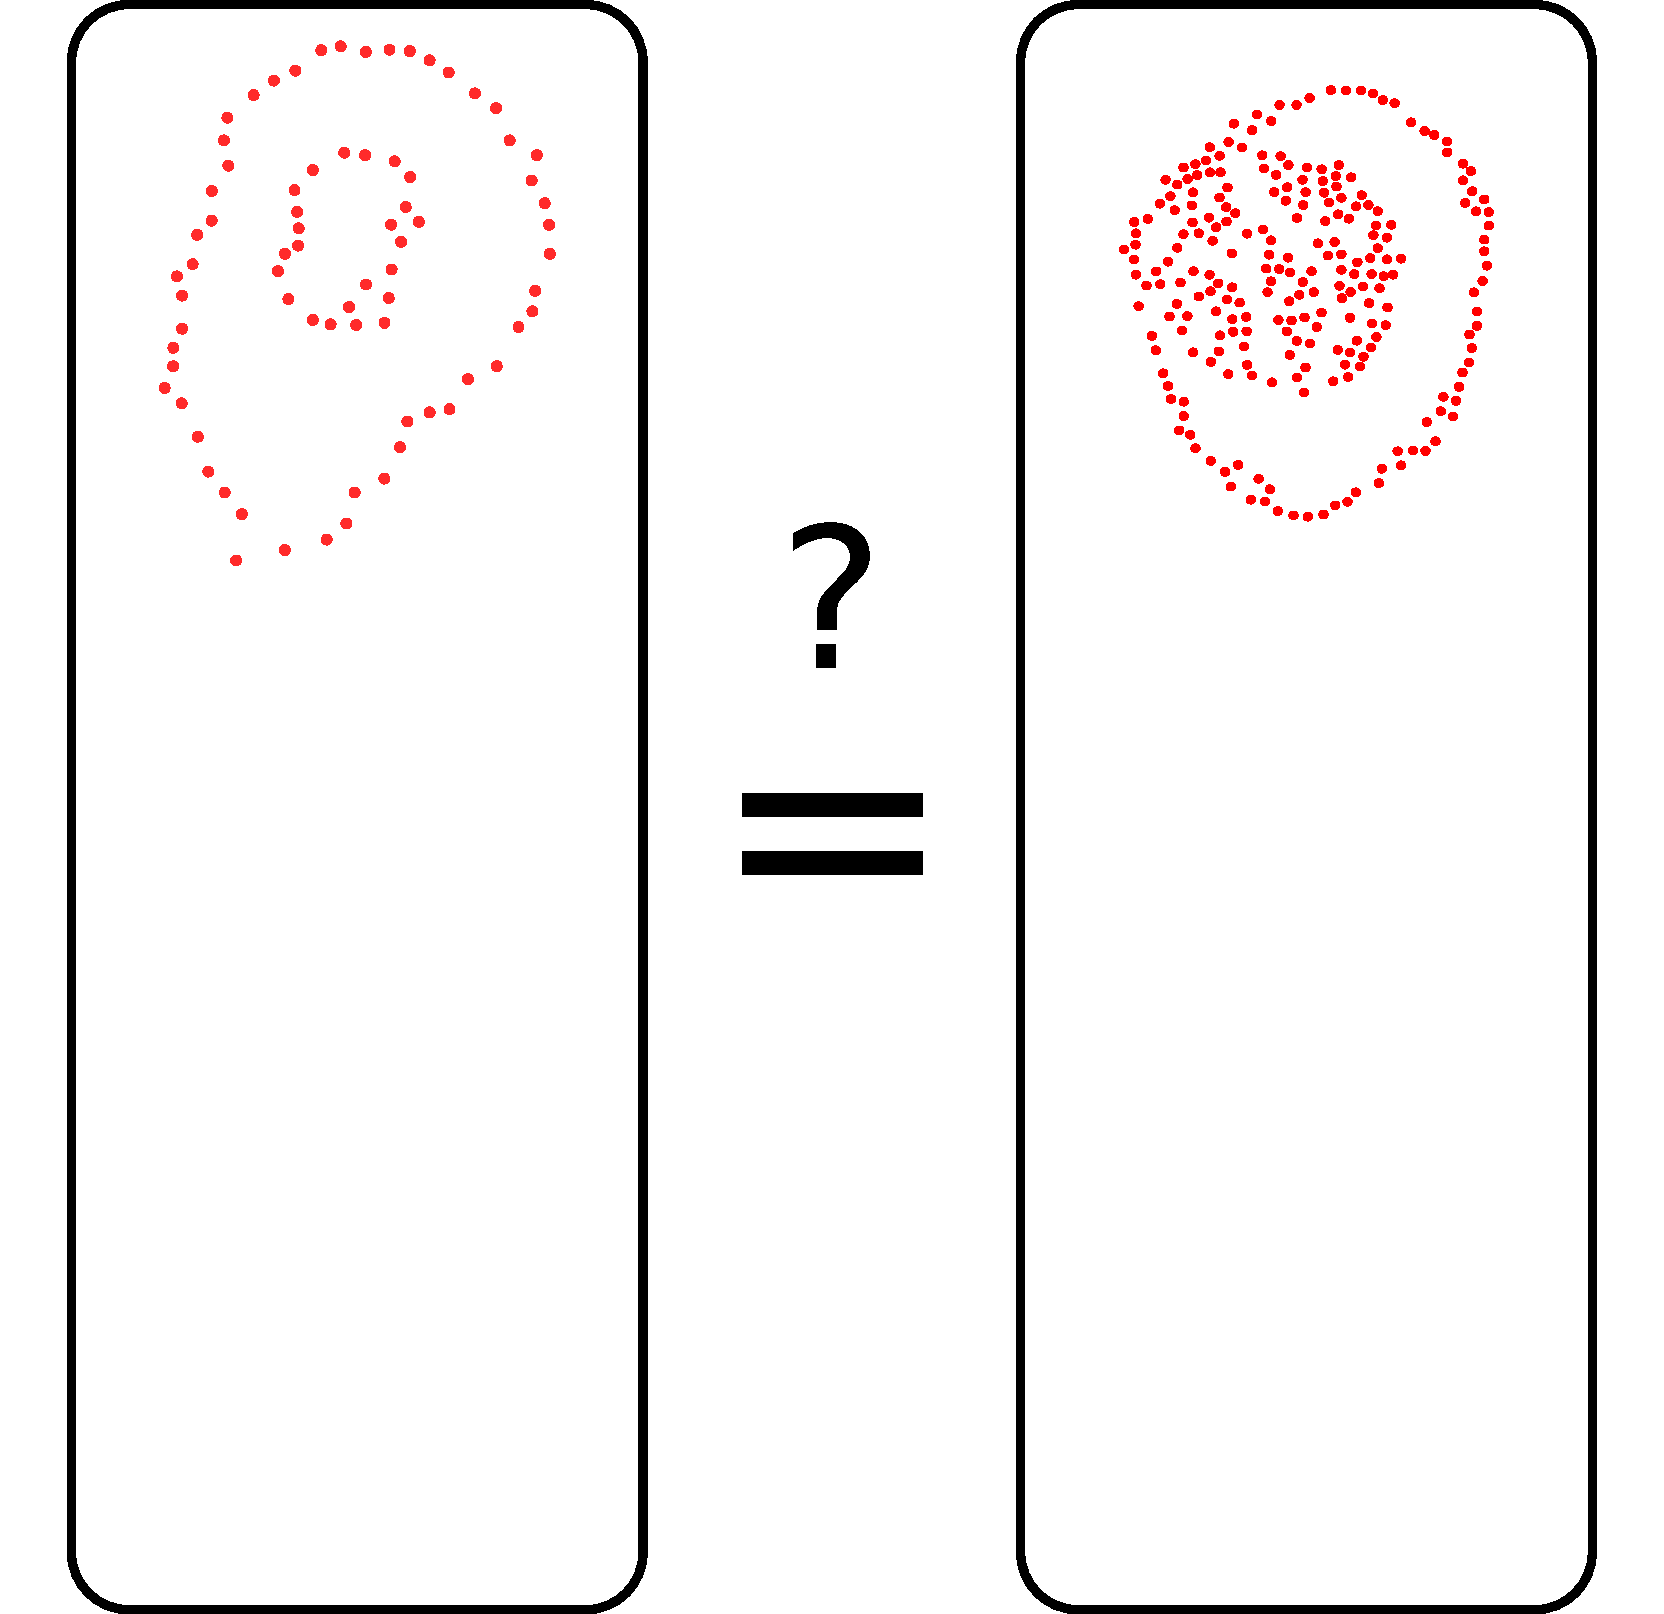
\includegraphics[width=.7\textwidth]{topology/inference-compare-1}}%
 \only<2->{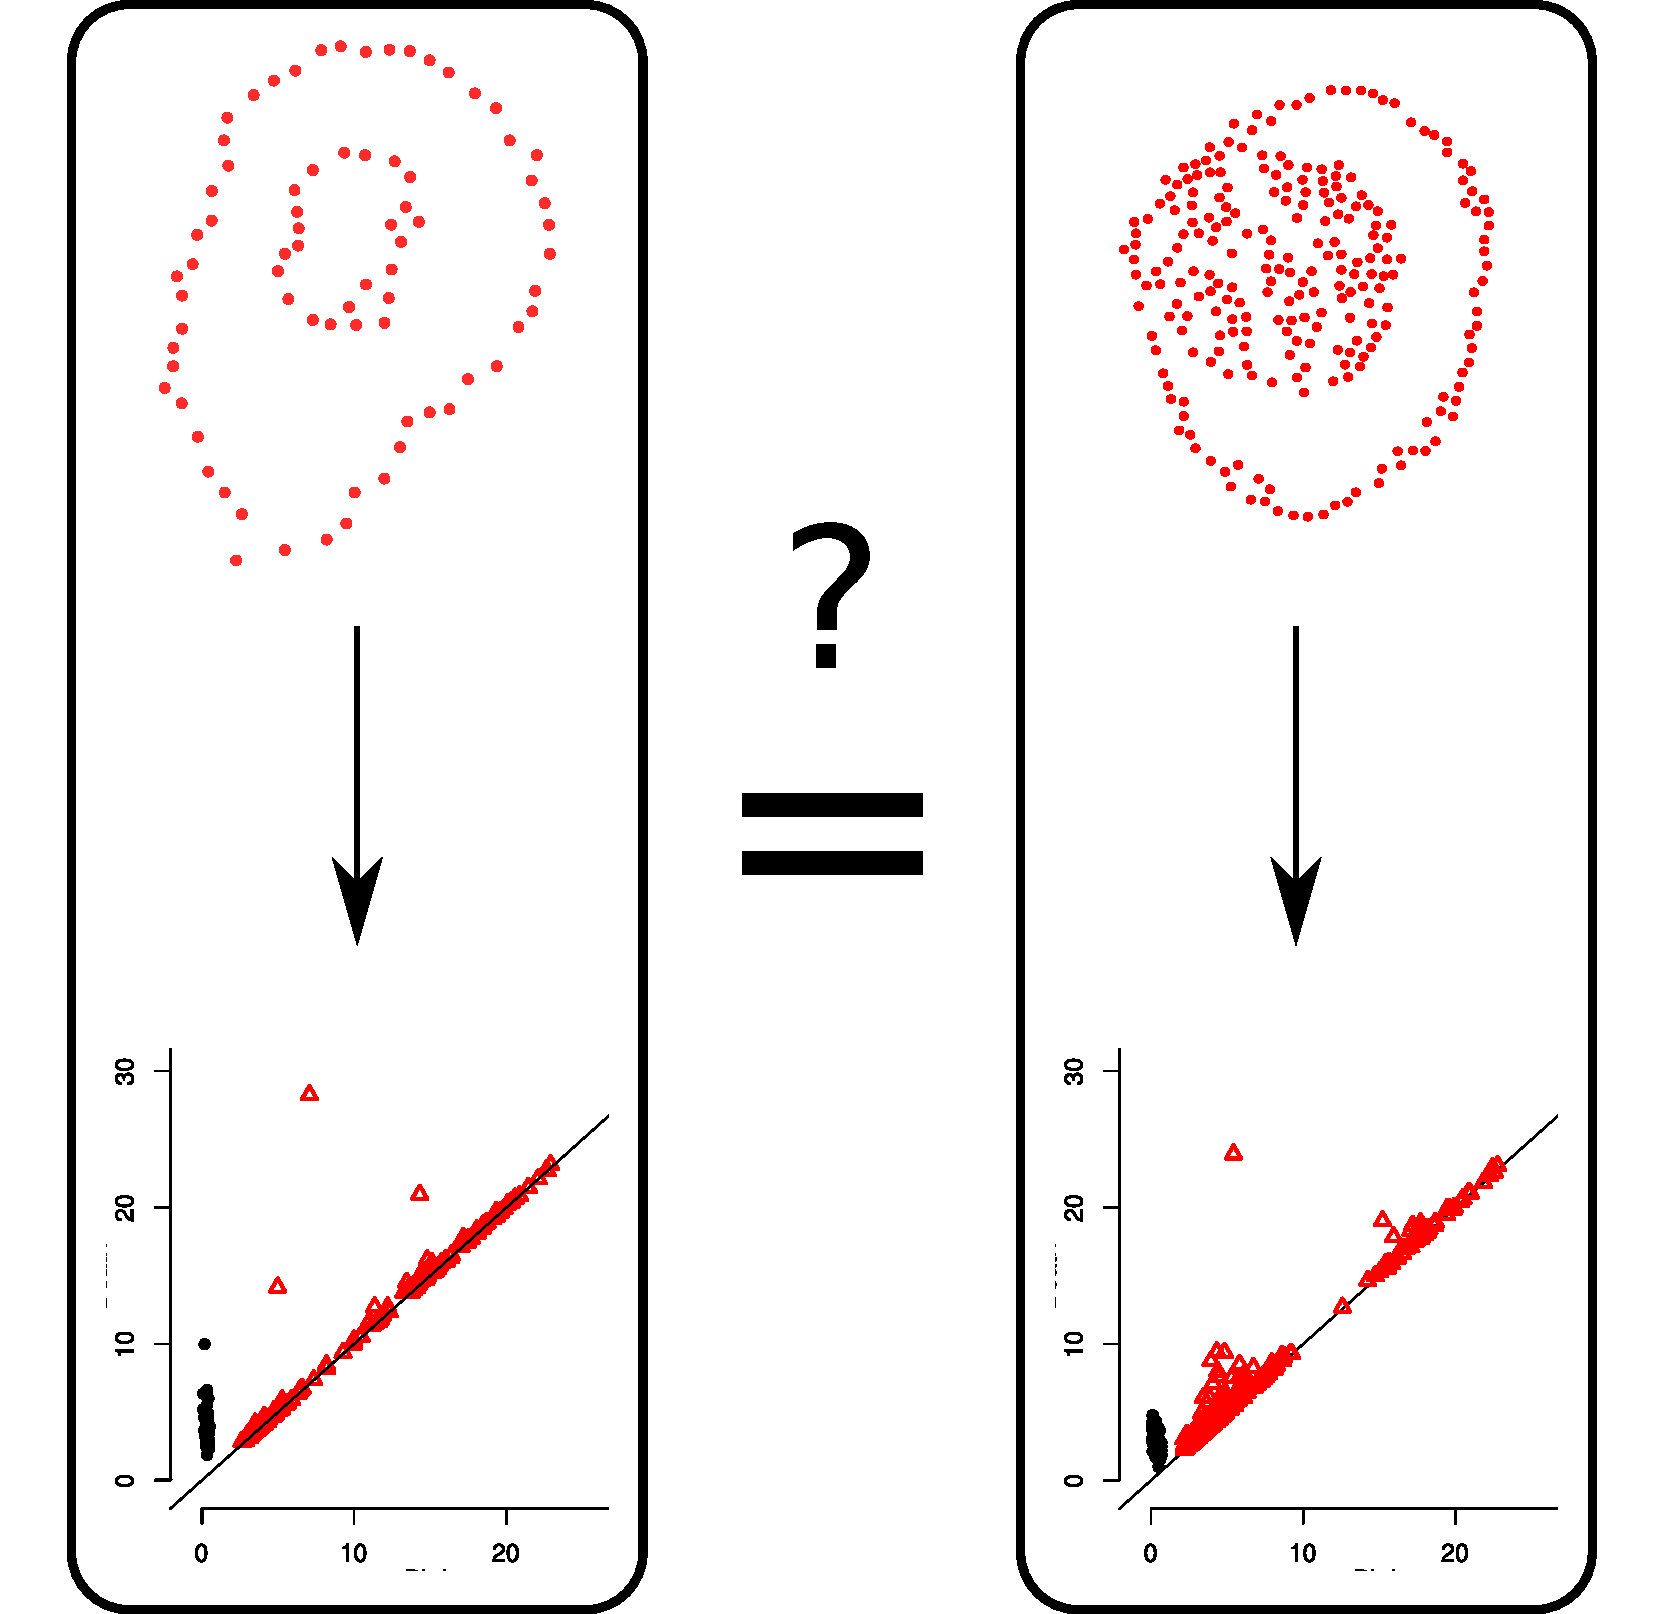
\includegraphics[width=.7\textwidth]{topology/inference-compare-2}}%
\end{block}

}


\frame{
    \frametitle{Distances Between Diagrams}
    \begin{columns}%
        \column{.45\textwidth}
        \begin{block}{}
            \onslide<1->{
                \begin{itemize}
                    \item Bottleneck $d_{\infty}$.
                    \item Interleaving distance.
                    \item Wasserstein $d_p$.
                    \item Erosion distance.%
                \end{itemize}%
            }%
        \end{block}%
%
        \pause%
        \begin{block}{Question}%
            Can we define a centroid / Fr\'echet mean?
            $$ \arg\min_D \sum_i W^2_{\infty}(D,D_i)$$
        \end{block}%
%
            \pause
            \column{.45\textwidth}
        \begin{block}{}
            \centering
            \only<2>{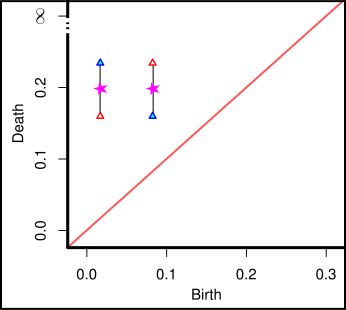
\includegraphics[height=1.9in]{stat/dgm-average}}%
            \only<3>{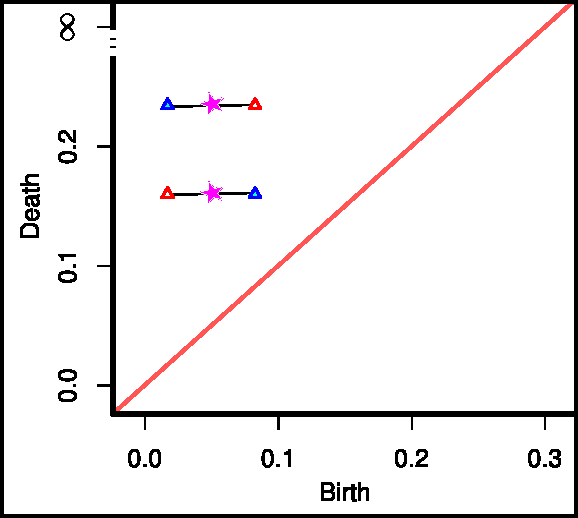
\includegraphics[height=1.9in]{stat/dgm-average-opt1}}%
            \only<4->{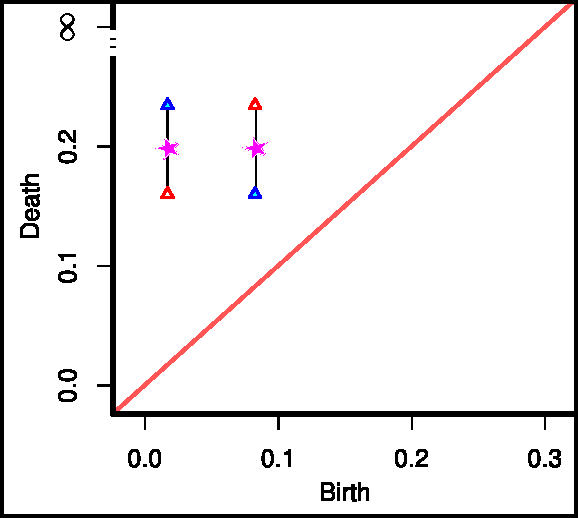
\includegraphics[height=1.9in]{stat/dgm-average-opt2}}%
        \end{block}

        \tiny{
        1. Turner, Mileyko, Mukherjee, and Harer. Fr\'echet Means for Distributions
        of Persistence Diagrams. DCG, 2014.\\
        2. Munch, Tuner, Bendich, Mukherjee, Mattingly, and Harer.
        Probabilistic Fr\'echet Means for Time Varying Persistence Diagrams.
        Electronic Journal of Statistics, 2015.
    }

    \end{columns}
}

\frame{
\begin{block}{}
\centering
 \only<1>{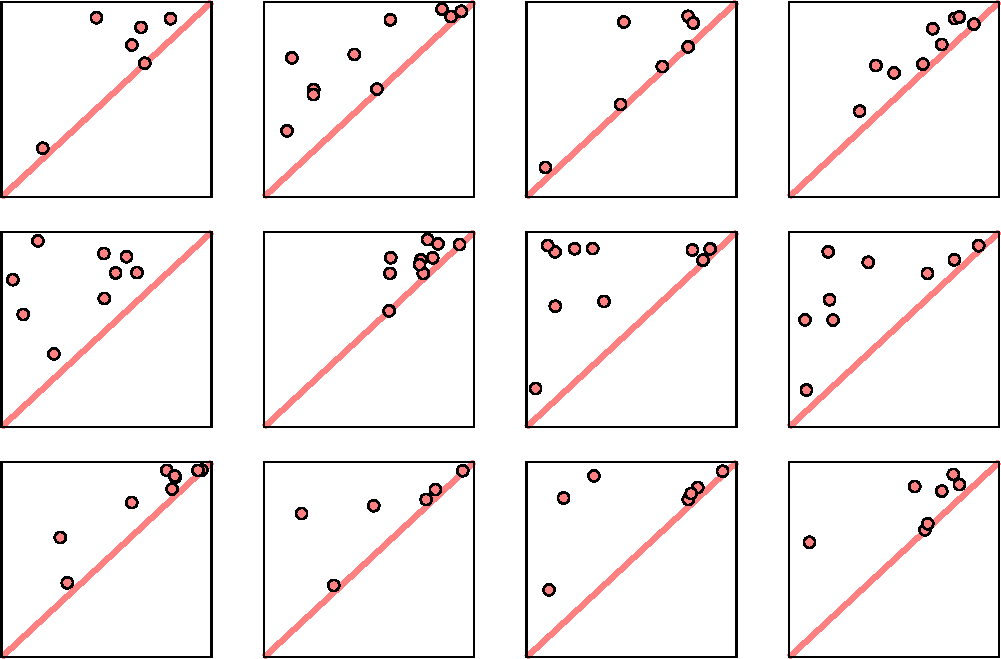
\includegraphics[width=.7\textwidth]{stat/sampling-dgms}}%
 \only<2->{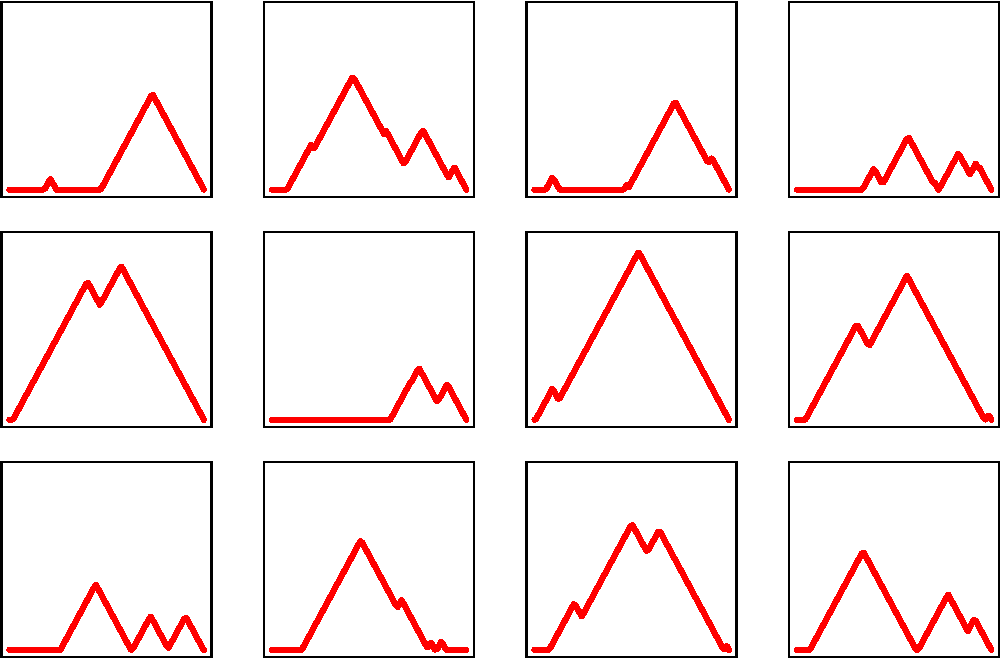
\includegraphics[width=.7\textwidth]{stat/sampling-lscapes}}%
\end{block}

}

\frame{

\begin{block}{}
    \centering
   Clustering
\end{block}
}

\frame{
    \frametitle{Clustering
    \onslide<5->{... and Classification} }

    \begin{block}{Clustering (Unsupervised Learning)}
        \pause
        \begin{itemize}
            \item Heirarchical: agglomerative or divisive.\pause
            \item $k$-means: NP-hard, so algorithms find a local minimum.
            \item Distribution- and density-based clustering: e.g., DBSCAN.
                \pause
            \item Fuzzy clustering: membership is not binary.
        \end{itemize}
    \end{block}

    \pause%
    \begin{block}{Classification (Supervised Learning)}
        input data (training sample): $D=\{(X_i,Y_i)\}_{i=1}^n$\\~\\
        $k$-nn clustering: for new $X$, we predict $Y$ by majority vote of the
        $k$ nearest neighbors of the covariates (features) in $D$.
    \end{block}
}

\begin{frame}

\frametitle{Homework!}

\begin{block}{}
Curate a list of topological descriptors.  For each, we are looking for:
\begin{itemize}
\item Name of descriptor
\item Short explanation (very short)
\item Reference to where first used (if possible)
\item Pros: What is it good for?
\item Cons: Where / when is it insufficient?
\end{itemize}
\end{block}
\todo{Sam, can you create a wiki page for this that perhaps they can edit
directly as we are in class during the second day?}

\end{frame}


%% Day 2
\begin{frame}
\subtitle{Part II}
\titlepage
\end{frame}

\frame{
    \begin{block}{Today's Lecture}
        \begin{itemize}
            \item Functional summaries.
            \item Review HW.
            \item Application.
        \end{itemize}
    \end{block}
}

%
%%%%%%%%%%%%%%%%%%%%%%%%%%%%%%%% FUNCTIONAL SUMMARIES


\frame{
\frametitle{}
\begin{block}{}
\centering
Functional Summaries and Their Confidence Sets
\end{block}
}

\frame{
    \frametitle{Applications (of Functional Summaries)}
    \framesubtitle{Thanks, Lisbeth!}

\begin{columns}
    \column{.45\textwidth}
    \begin{block}{A Sample of Summaries}
        \begin{itemize}
            \item Variance
            \item Mean Computation
            \item Confidence Bands
            \item Functional Boxplots
        \end{itemize}
    \end{block}
    \column{.45\textwidth}
    \begin{block}{Two Samples of Summaries}
        \begin{itemize}
            \item Two-sample Hypothesis Test
            \item Paired Hypothesis Test
            \item Clustering
            \item Supervised Classification
        \end{itemize}
    \end{block}
\end{columns}
}

\frame{
\frametitle{Eyeballing the Distribution}

\begin{block}{}
  \centering
  \only<1>{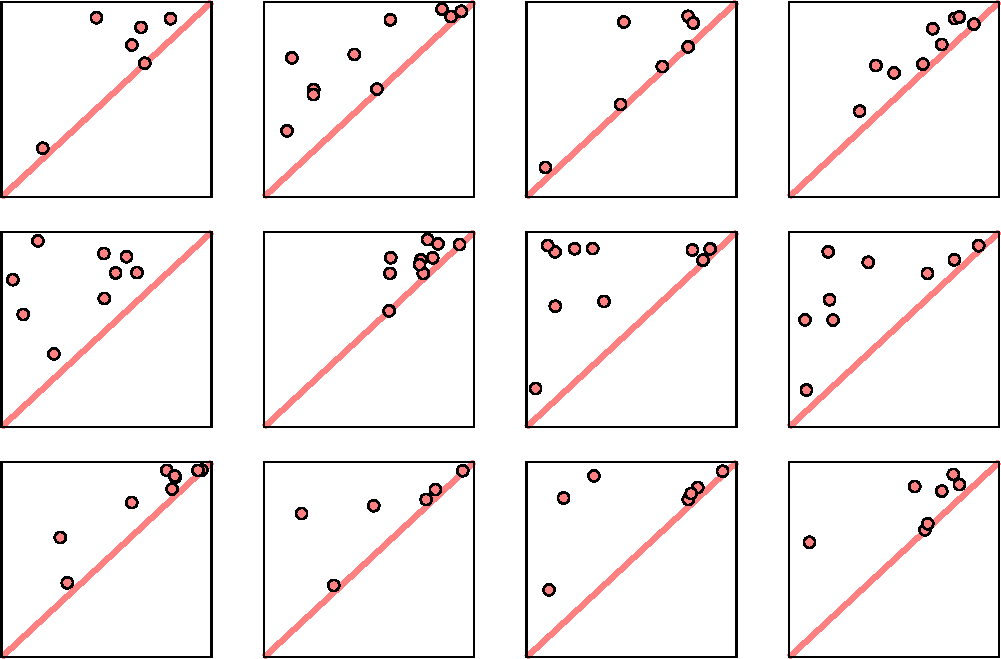
\includegraphics[height=2in]{stat/sampling-dgms}}%
  \only<2>{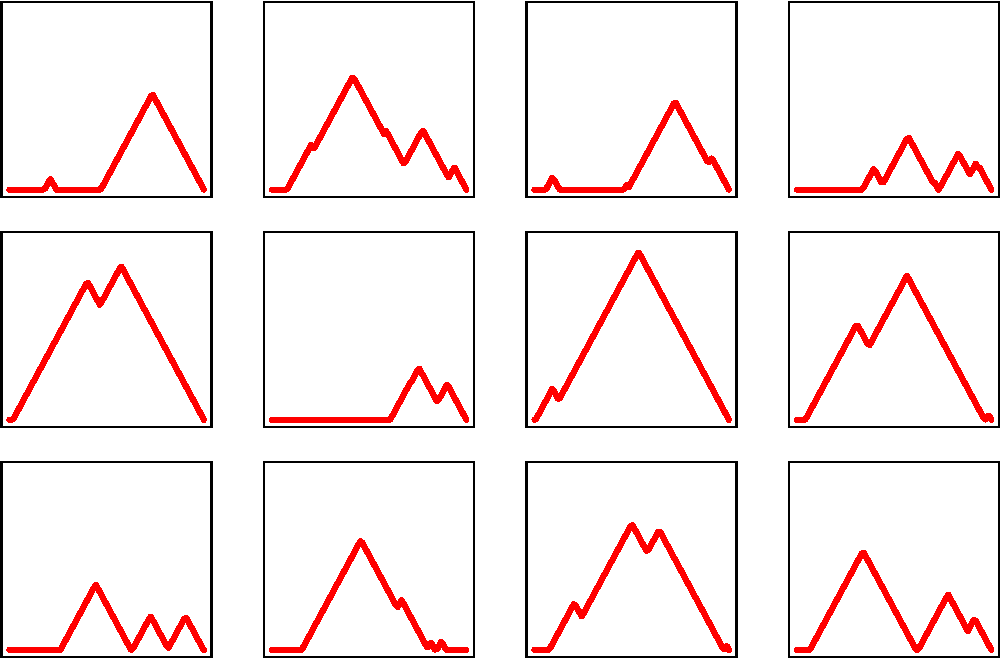
\includegraphics[height=2in]{stat/sampling-lscapes}}%
\end{block}

}

\frame{
\frametitle{Persistence Landscapes}
\framesubtitle{
    \onslide<3->{    Bubenik. Statistical topological data analysis using persistence landscapes,
JMLR, 2015.}}

\begin{center}
\only<1>{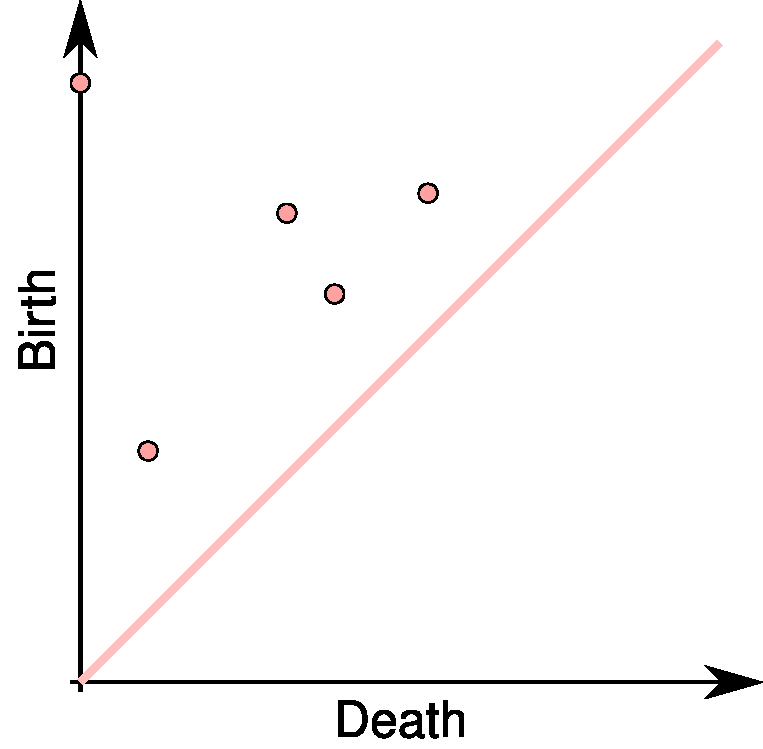
\includegraphics[height=2in]{stat/persistence-dgm}}%
\only<2>{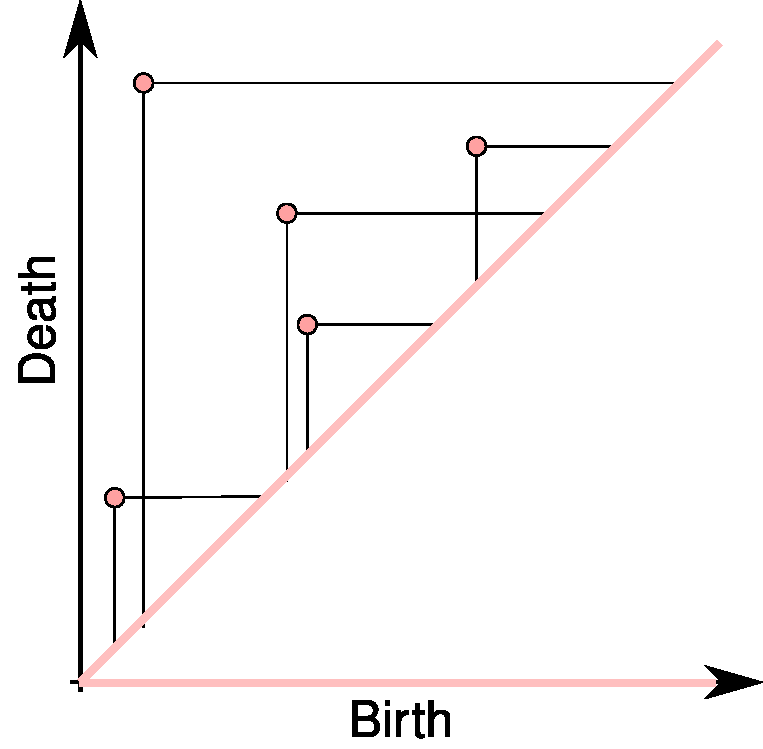
\includegraphics[height=2in]{stat/persistence-dgm-dropped}}%
\only<3>{\includegraphics[height=2in]{stat/persistence2-labeled}}%
\only<4->{\includegraphics[height=2in]{stat/persistence-lscape}}%
\end{center}
}

\frame{
    \frametitle{Persistence Landscapes and Silhouettes}
\begin{columns}
    \column{.45\textwidth}
    \begin{center}

        \only<1>{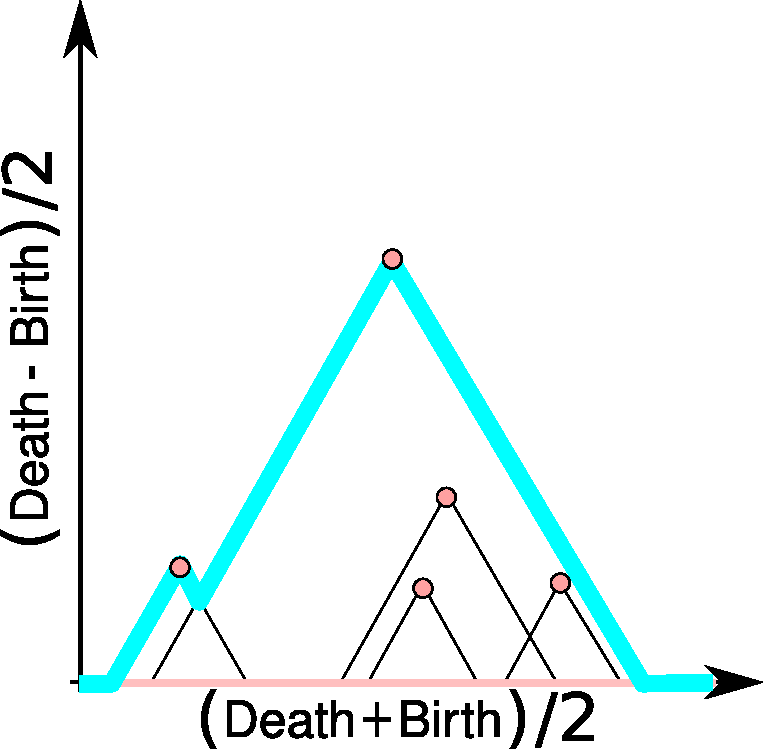
\includegraphics[height=2.5in]{stat/persistence-one-landscape}}%
        \only<2>{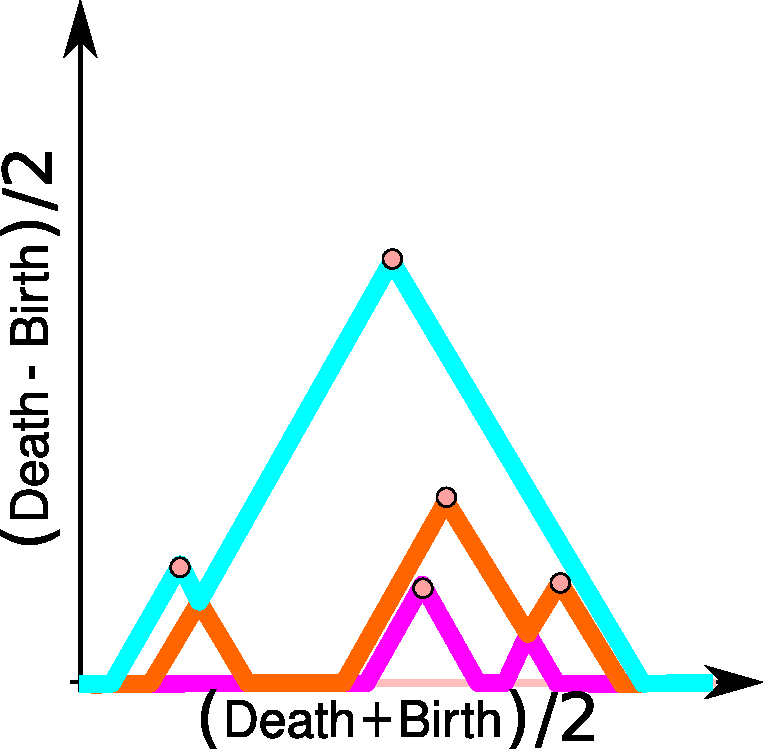
\includegraphics[height=2.5in]{stat/persistence-all-landscapes}}%
        \only<3>{\includegraphics[height=2.5in]{stat/persistence2-labeled}}%
        \only<4->{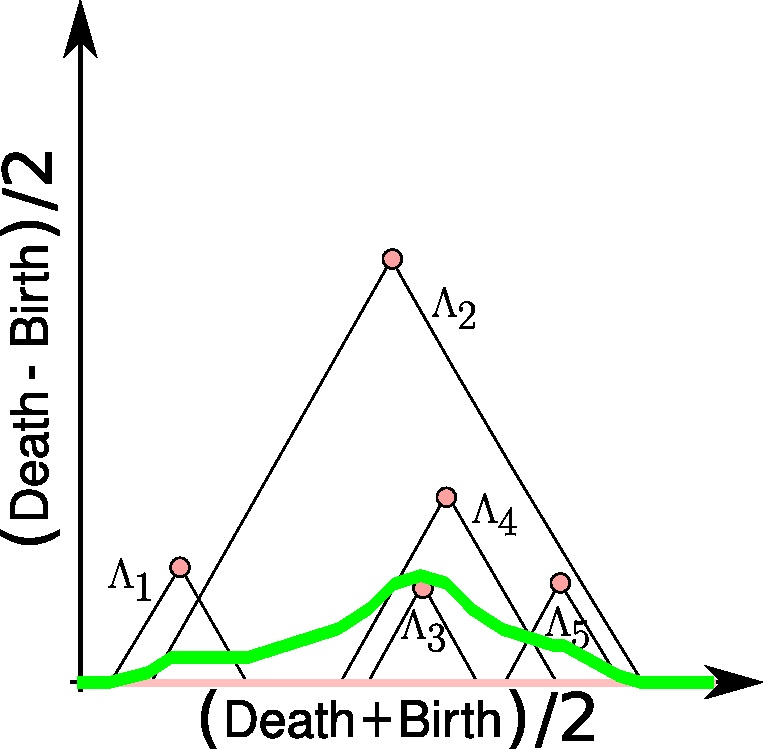
\includegraphics[height=2.5in]{stat/persistence-silhouette}}%
    \end{center}
    \column{.45\textwidth}

    \only<2>{
        \begin{block}{}
            $$\Lambda \colon \R \times \Z_{+} \to \R$$
            $$\Lambda_i(\cdot) := \Lambda(\cdot,i)$$
        \end{block}
    }

    \only<4->{
        \begin{block}{Weighted Silhouette}
            $$ \phi(t) = \frac{\sum_{i=1}^n w_i \Lambda_i(t) }{ \sum_{j=1}^n w_j} $$
        \end{block}
        \onslide<5>{
            \begin{block}{Power-Weighted Silhouette}
            $$w_i = |d_i - b_i|^p$$
            \end{block}
        }
    }%end only<4->

\end{columns}


}

\frame<1->{
\frametitle{Weak Convergence of Landscapes}
\begin{columns}
 \column{.45\textwidth}
    \begin{center}
    \only<1>{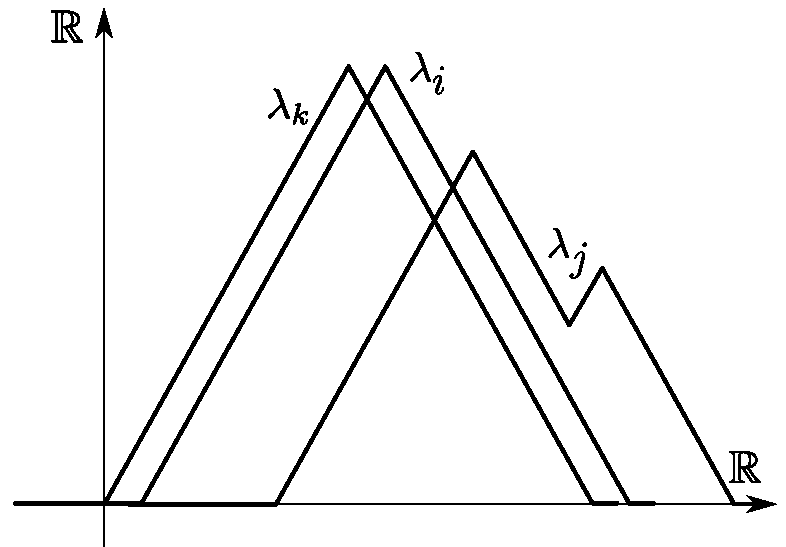
\includegraphics[width=\textwidth]{stat/gaussianprocess-lscapes}}%
    \only<2>{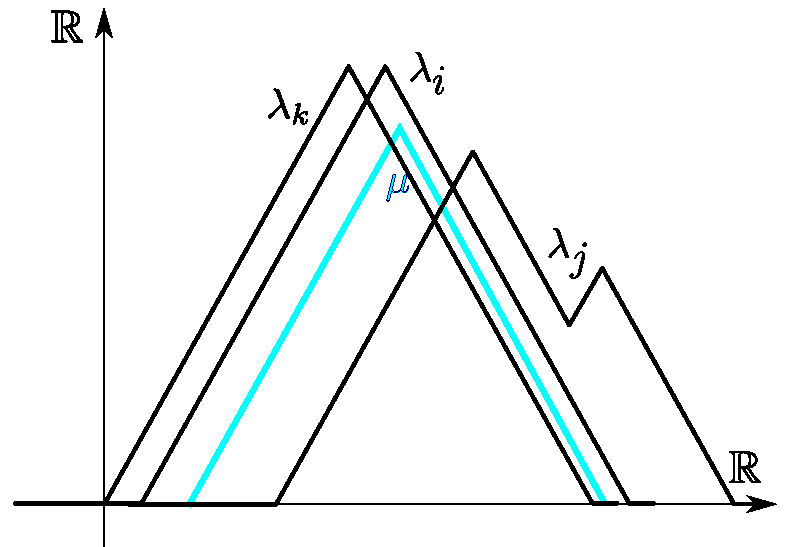
\includegraphics[width=\textwidth]{stat/gaussianprocess-mean}}%
\only<3>{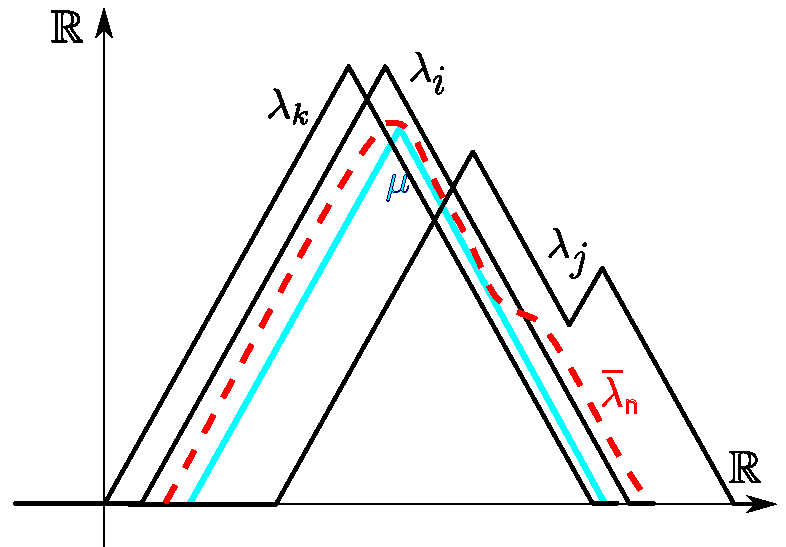
\includegraphics[width=\textwidth]{stat/gaussianprocess-empirical}}%
    \only<4->{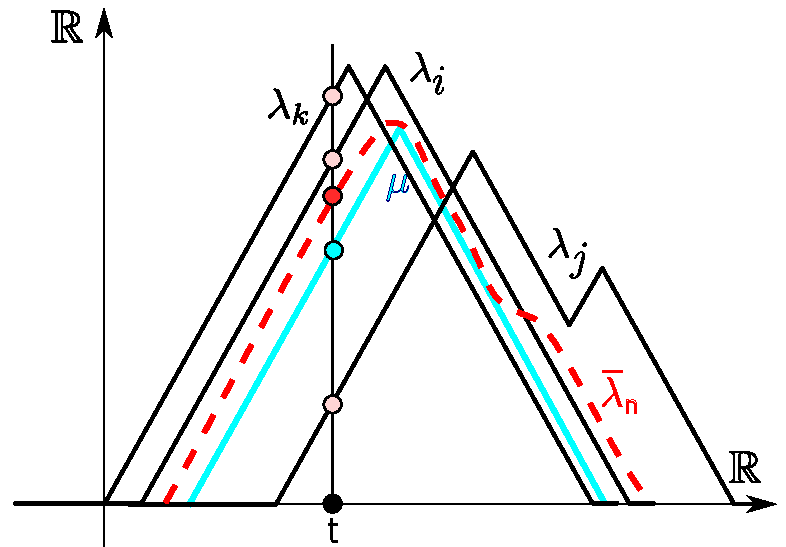
\includegraphics[width=\textwidth]{stat/gaussianprocess}}%
    \end{center}
 \column{.45\textwidth}
 \begin{block}{}
 Let $\lambda_1, \ldots, \lambda_n \sim \mathcal{L}_T$.\\ \pause
 $\lambda$ : true (unknown) landscape\\
  $\mu = \mathbb{E}(\lambda_i)  $\\ \pause
 $\bar{\lambda}_n$ : average landscape \pause
\end{block}
\end{columns}

\begin{block}{Pointwise Convergence  [B-2015 (JMLR), also arXiv:1207.6437].}
 {\color{red} $\bar{\lambda}_n$} converges pointwise to {\color{cyan} $\mu$}.
\end{block} \pause

% % \begin{block}{Gaussian Process on $[0,T]$}
% % For $t \in [0,T]$, we define
% % $ \mathbb{G}_n(f_t) = \mathbb{G}_n(t) := \frac{1}{\sqrt{n}}
% (\bar{\lambda}_n(t)
% % - \mu(t)
% % )$.
% % \end{block}

\begin{block}{Uniform CLT}
We proved this in [CFLRW-14 (SoCG), also arXiv:1312.0308].
\end{block}


} % end frame



\frame{
\frametitle{{Asymptotic} Confidence Bands}
 \begin{columns}
 \column{.45\textwidth}
    \begin{center}
    \only<0>{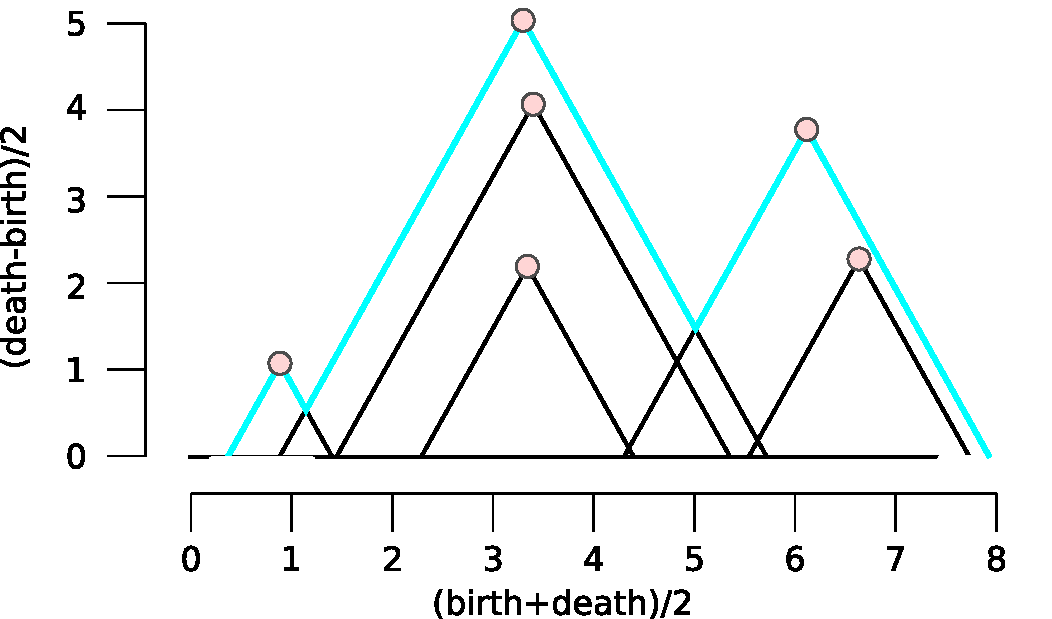
\includegraphics[width=\textwidth]{stat/triangles3b}}%
    \only<1-2>{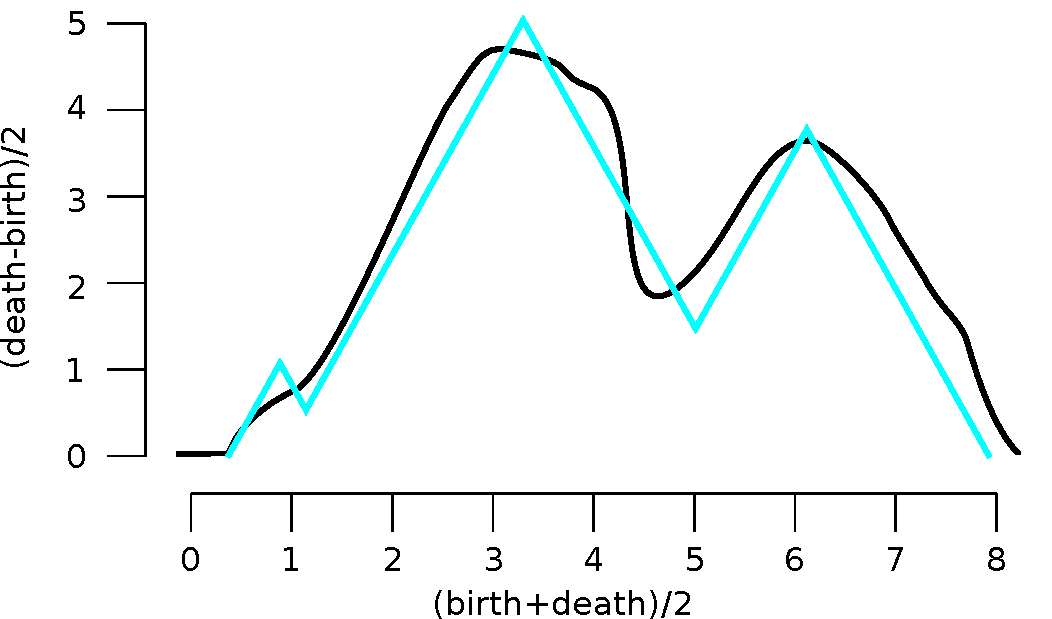
\includegraphics[width=\textwidth]{stat/triangles-avg}}%
    \only<3->{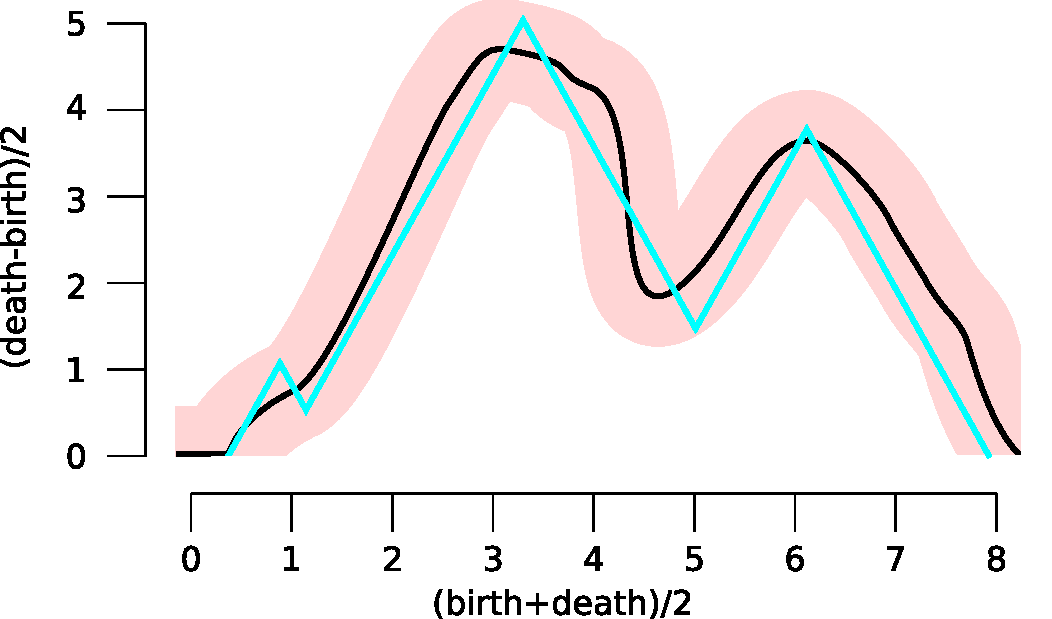
\includegraphics[width=\textwidth]{stat/triangles-CI}}%
    \end{center}
 \column{.45\textwidth}
    \begin{block}{}
    \begin{eqnarray*}
    \mathbb{E}||\lambda -\bar{\lambda}_n||_{\infty}
    &\leq&
    \overbrace{\mathbb{E}||\mu
    -\bar{\lambda}_n||_{\infty}}^{\text{variance}}\\
    \onslide<1>{&& + \underbrace{\mathbb{E}||\lambda - \mu
    ||_{\infty}}_{\text{bias}} \\ }
    \end{eqnarray*}
    \end{block}
 \end{columns}


\onslide<3->{
\begin{block}{\onslide<3->{Asymptotic} Confidence Band}
Find $c$ such that $\ell_n = \bar{\lambda}_n - c$ and
$u_n = \bar{\lambda}_n + c$ such that
$$
\only<3->{\lim_{n\to \infty}}
\mathbb{P}(\ell_n(t) \leq \mu(t) \leq u_n(t) \text{ for all } t)
\geq 1 - \alpha.
$$
\end{block}
}% end onslide
}% end frame


\frame<2>{
\frametitle{Confidence Bands for Landscapes}
\framesubtitle{Via the Multiplier Bootstrap}
\begin{block}{}
 $\xi_1, \ldots, \xi_n \sim N(0,1)$\\
 $$\widetilde{\mathbb{G}}_n(f_t) := \frac{1}{\sqrt{n}}
 \sum_{i=1}^n \xi_i (\lambda_i(t) - \bar{\lambda}_n (t))$$
\end{block}

\begin{columns}
\column{.45\textwidth}
  \begin{block}{$\alpha$-Quantile}
  $\widetilde{Z}_{\alpha}$ is the unique value such that
  $$
  \mathbb{P} \left( \sup_{t} | \widetilde{\mathbb{G}}_n(f_t) | >
\widetilde{Z}_{\alpha}  \Biggm| \{ \lambda_i \} \right) = \alpha
  $$
  \onslide<2->{*Approx. $\widetilde{Z}_{\alpha}$ by MC
simulation}
  \end{block}
\column{.45\textwidth}
  \only<1>{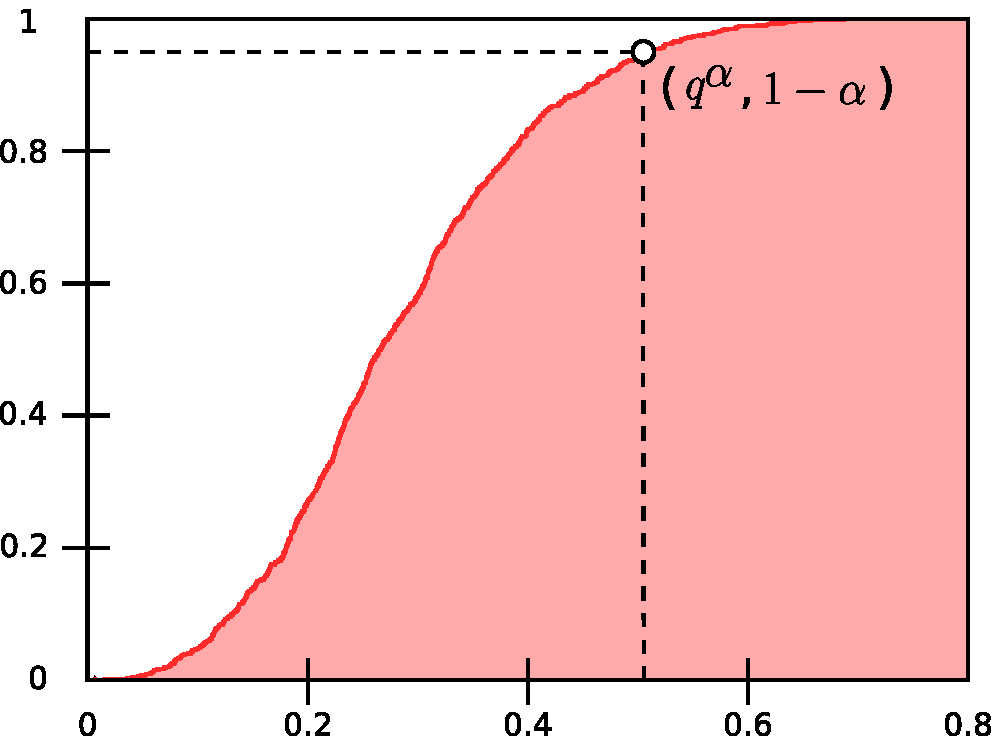
\includegraphics[width=0.75\textwidth]{stat/cdf-full}}%
  \only<2->{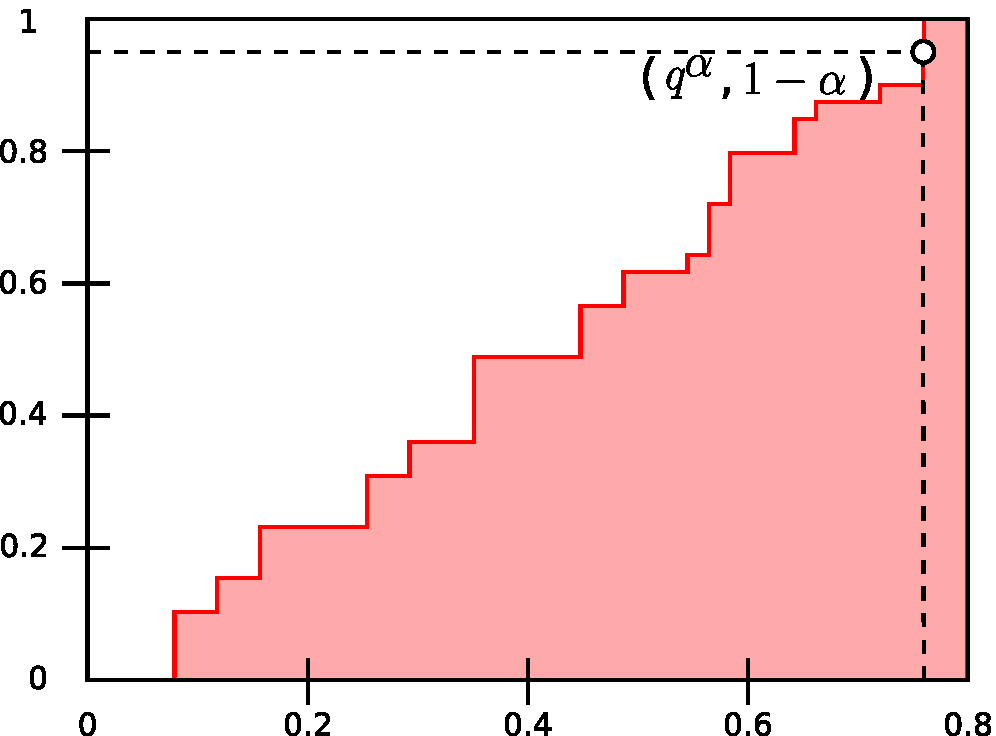
\includegraphics[width=0.75\textwidth]{stat/cdf-discrete}}%
\end{columns}
}

\frame{
\frametitle{Confidence Bands for Landscapes}
\framesubtitle{The Uniform Band}
\begin{columns}
\column{.45\textwidth}
\begin{block}{}
 $$ \ell_n = \bar{\lambda}_n(t) - \frac{\tilde{Z}(\alpha)}{\sqrt{n}}$$
 $$   u_n = \bar{\lambda}_n(t) + \frac{\tilde{Z}(\alpha)}{\sqrt{n}}$$
\end{block}

\column{.45\textwidth}
  \only<1->{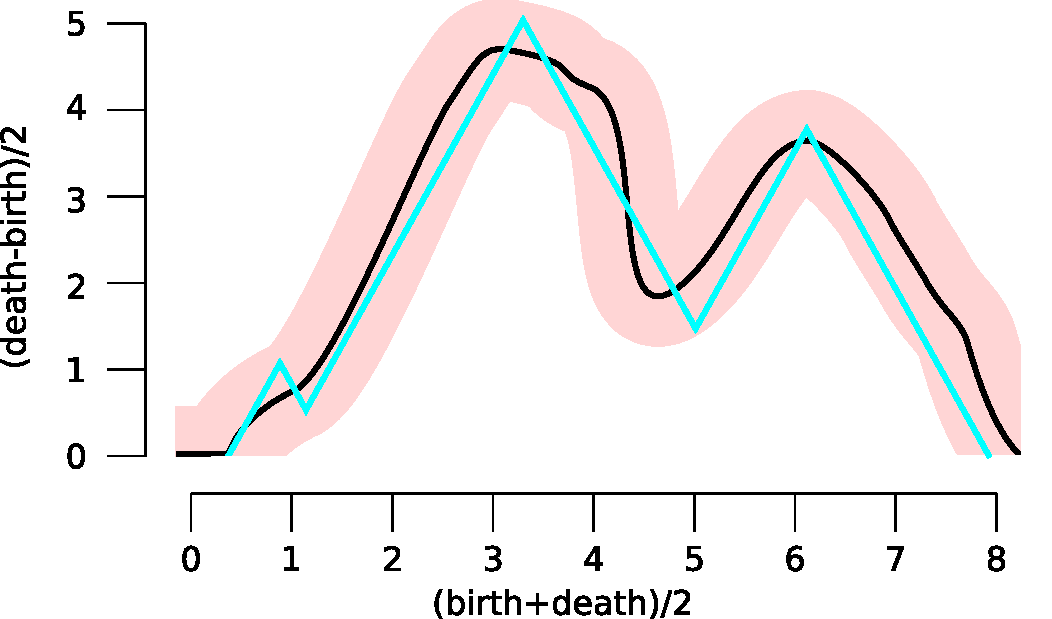
\includegraphics[width=0.75\textwidth]{stat/triangles-CI}}%
\end{columns}

\begin{block}{Uniform Band}
 $$
    \mathbb{P} \left( \ell_n(t) \leq \mu(t) \leq u_n(t)
    \text{ for all } t \right)
    \geq 1 - \alpha
    - \Big( \frac{(\log n)^{\frac{7}{8}} }{n^{\frac{1}{8}}}\Big).
 $$
\end{block}
}

\section{Functional Summaries}
\frame{
\frametitle{Functional Summaries}
\framesubtitle{~}

\begin{block}{}
\begin{itemize}
 \item Persistence Landscapes.
 \item Silhouettes.
 \item Maximum persistence.
 \item Euler characteristic curve.
 \item Accumulated Persistence Function (APF).
 \item Betti numbers.
 \item Birth (or death times) of persistence points.
\end{itemize}
\end{block}


---------------------------------\\
{Berry, Chen, Cisewski, and Fasy.  One dimensional topological
    descriptors. Coming soon!!}

}

\section{Listing Descriptors}
\againframe<1>{firsthw}

\begin{frame}
    \begin{block}{}
        \centering{Homework Review}
    \end{block}
\end{frame}

\frame<1>[label=secondhw]{
\frametitle{Homework Review!}

\begin{block}{}
    \begin{itemize}
\item Pair: In groups of 2-3, discuss your lists. (6 min) \pause
\item Share: In groups of 5-9, add to Padlet (6 min)
    \end{itemize}
\end{block}

}

\againframe<1>{firsthw}

\againframe<1->{secondhw}
\againframe<2>{firsthw}

%\input{body/roads}

%\section{Conclusion}
\frame{
    \frametitle{Announcements}

    \begin{block}{}
        \begin{itemize}
            \item \url{WinCompTop+subscribe@googlegroups.com} \pause
            \item R Package TDA (BTF, J.\ Kim, F.\ Lecci, C.\ Maria, D.\
                Millman, V.\ Rouvreau):
                \url{https://github.com/compTAG/r-tda} \pause
            \item We welcome students! (summer REU? PhD in CS or math? Visitor?) \pause
            \item
                This material is based upon work supported by
                the National Science Foundation under Grant Number NSF CCF
                1618605, and
                the National
                Institutes of Health and the National Science Foundation under
                Grant Numbers NSF DMS 1664858.
        \end{itemize}
    \end{block}
}



\begin{frame}
\frametitle{Thank You!}

    \centering
    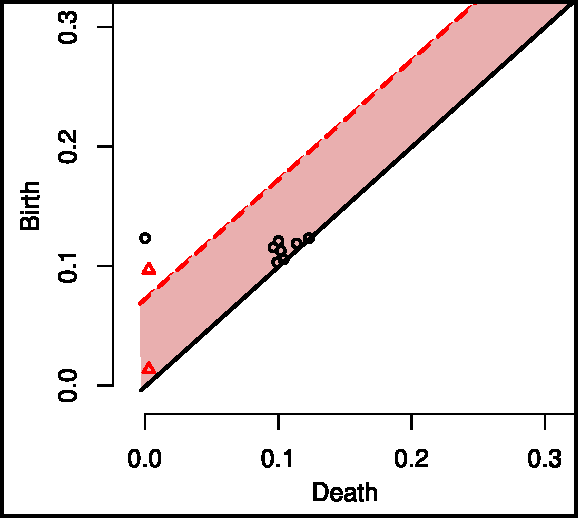
\includegraphics[width=.25\textwidth,height=1.25in]{stat/eyeglasses-density-pers-CI}~~
    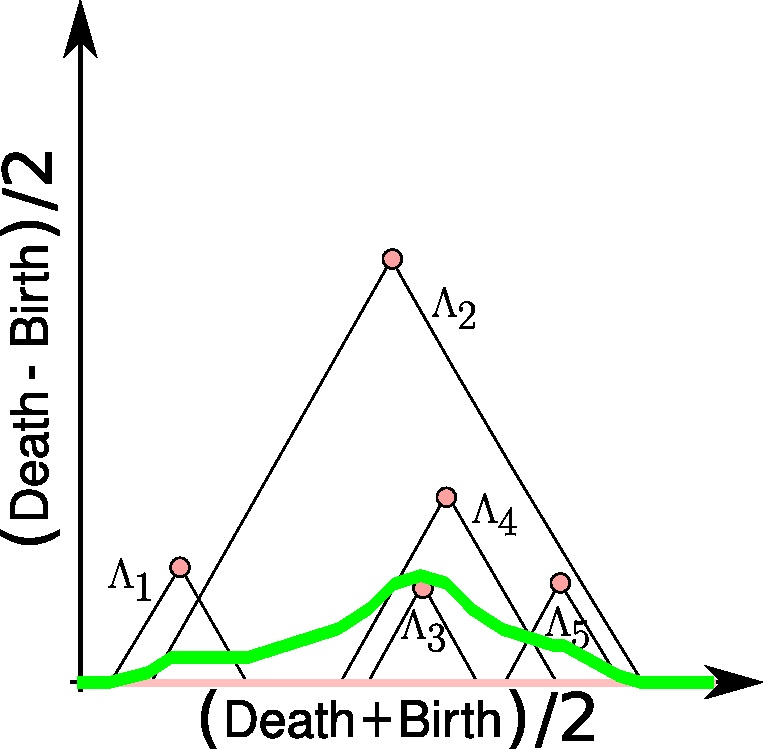
\includegraphics[width=.25\textwidth,height=1.25in]{stat/persistence-silhouette}~~
    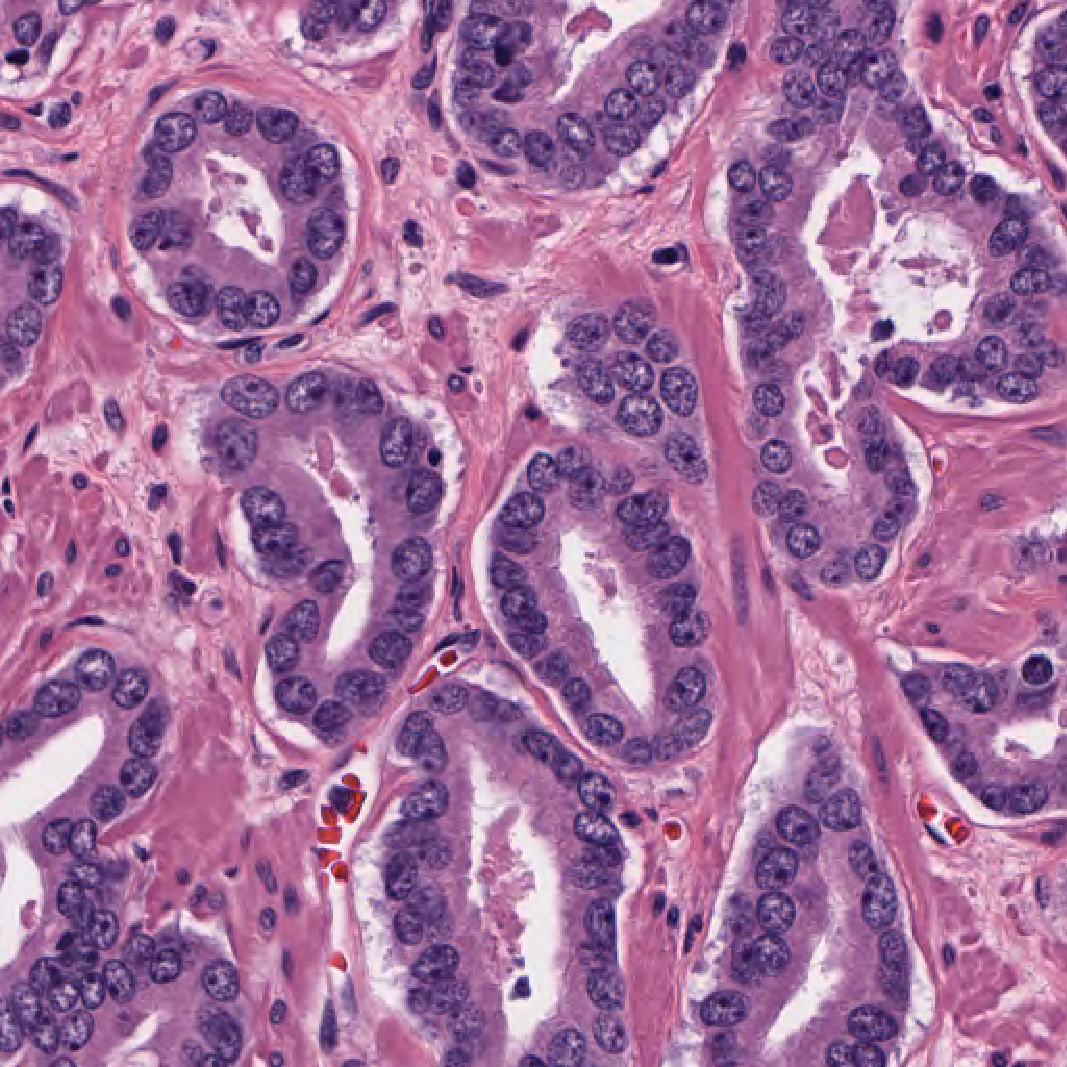
\includegraphics[width=.25\textwidth,height=1.25in]{gleason/gleason3}

    \begin{block}{}
        \centering
        Brittany: \url{brittany@fasy.us}\\
        Sam: \url{mickas37@gmail.com}
    \end{block}
\end{frame}


\end{document}
